\documentclass[11pt, spanish, a4paper, twoside]{article}
% LTeX: language=es-AR

% Versión 1.er cuat 2021 Víctor Bettachini < vbettachini@unlam.edu.ar >

\usepackage[T1]{fontenc}
\usepackage[utf8]{inputenc}

\usepackage[spanish, es-tabla]{babel}
% \def\spanishoptions{argentina} % Was macht dass?
% \usepackage{babelbib}
% \selectbiblanguage{spanish}
% \addto\shorthandsspanish{\spanishdeactivate{~<>}}


\usepackage{graphicx}
\graphicspath{{./figuras/}{../LaTeX/}{../referencia/figurasLaTeX/}{./figs}}
% \usepackage{float}

\usepackage[arrowdel]{physics}
\newcommand{\pvec}[1]{\vec{#1}\mkern2mu\vphantom{#1}}
\usepackage{isotope} % $\isotope[A][Z]{X}\to\isotope[A-4][Z-2]{Y}+\isotope[4][2]{\alpha}

% \usepackage{units}
\usepackage[
  separate-uncertainty= true,
  multi-part-units= single,
  range-units= single,
  range-phrase= {~a~},
  locale= FR,
  exponent-product= \cdot,
  ]{siunitx}
\DeclareSIUnit\atm{atm}
\DeclareSIUnit\kgf{kgf}

% \usepackage{enumerate}
\usepackage{tasks}
\usepackage[inline]{enumitem}

\usepackage{hyperref}
\usepackage{xcolor}

% \usepackage{amsmath}
% \usepackage{amstext}
% \usepackage{amssymb}

\usepackage{tikz}
\usepackage{tikz-3dplot}
\usepackage{tikz-dimline}
\usetikzlibrary{calc}
% \usetikzlibrary{math}
\usetikzlibrary{arrows.meta}
\usetikzlibrary{snakes}
\usetikzlibrary{decorations}
\usetikzlibrary{decorations.pathmorphing}
\usetikzlibrary{patterns}

\usepackage[hmargin=1cm,vmargin=3cm, top= 0.75cm,nohead]{geometry}

\usepackage{lastpage}
\usepackage{fancyhdr}
\pagestyle{fancyplain}
\fancyhf{}
\setlength\headheight{28.7pt} 
\fancyhead[LE, LO]{\textbf{Mecánica Analítica Computacional} }
% \fancyhead[LE, LO]{\textbf{Mecánica General} }
\fancyhead[RE, RO]{\href{https://ingenieria.unlam.edu.ar/}{$\vcenter{\hbox{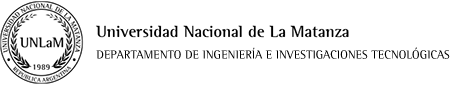
\includegraphics[height=1cm]{ingenieria_logo_schwarz.png}}}$}}
% \fancyhead[RE, RO]{\href{https://ingenieria.unlam.edu.ar/}{$\vcenter{\hbox{
\includegraphics[height=1cm]{ambos.pdf}}}$}}
\fancyfoot{\href{https://creativecommons.org/licenses/by-nc-sa/4.0/deed.es_ES}{$\vcenter{\hbox{
\includegraphics[height=0.4cm]{by-nc-sa_80x15.pdf}}}$} \href{https://ingenieria.unlam.edu.ar/}{DIIT - UNLaM}}
\fancyfoot[C]{ {\tiny Actualizado al \today} }
\fancyfoot[RO, LE]{Pág. \thepage/\pageref{LastPage}}
\renewcommand{\headrulewidth}{0pt}
\renewcommand{\footrulewidth}{0pt}

\begin{document}
\begin{center}
  % \textsc{\large Mecánica general}\\
  \textsc{\large Fuerzas de ligadura | Multiplicadores de Lagrange} 
\end{center}

\begin{enumerate}

	\item
	% \begin{minipage}[t][3.5cm]{0.7\textwidth}
	\begin{minipage}[t][0cm]{0.7\textwidth}
		\textbf{Péndulo rígido ideal}\\
		Calcule la tensión de la cuerda con el método de multiplicadores de Lagrange.
		La restricción es que la pesa se mantiene siempre en \(\vec{r} = \ell \hat{\rho}\), ergo la función que expresa esto es \(f(\rho) = \rho - \ell = 0\).
	\end{minipage}
	\begin{minipage}[c][0cm][t]{0.25\textwidth}
			\begin{tikzpicture}[scale= 1.3]
  	\draw [arrows=-latex] (-1,2) -> (-1,1) node [above=15, right=2] {\(\vec{g}\)}; % g vertical
		\draw [ultra thick] (-1.5,3) -- (2,3);
		\fill [pattern = north east lines] (-1.5,3) rectangle (2,3.2); % techo
		\draw [dashed] (0,3) -- (0,-.25);	% vertical
		\draw [thick] (0,3) -- +(-60:3) node[midway,above,right=2] {\(\ell\)};	% inclinada +:relativa, -60 grados, longitud 3
		\shade [ball color=black!80] ($(0,3)+(-60:3)$) circle(0.25) node [] {\color{white} $m$};
    %\draw [arrows=-latex] (0,.4) -> (1.25,.4) node [midway, above] {\( \psi \)}; % desplazamiento horizontal
		\draw [arrows=-latex] (0,0) arc [start angle=-90, end angle=-65, radius=3] node [below=12, left=8] {\( \varphi \)};
	\end{tikzpicture}
	\end{minipage}



	\item 
	\begin{minipage}[t][3cm]{0.47\textwidth}
	\textbf{Cilindro que rueda por un plano inclinado} [Marion (e) ex. 7.5]\\
	% English \textbf{Marion ejemplo 6.5 y ejemplo 7.9} Disco rodando en un plano inclinado.
		\begin{enumerate}
			\item Encuentre las ecuaciones de movimiento, 
			\item la aceleración angular,
			\item y la fuerzas de ligadura. 
		\end{enumerate}
	\end{minipage}
	\begin{minipage}[c][2cm][t]{0.3\textwidth}
		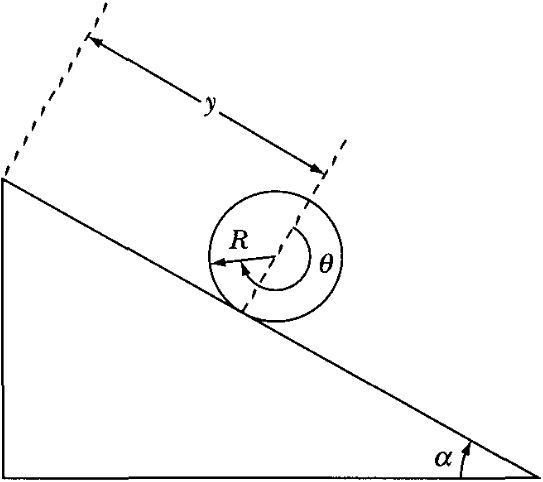
\includegraphics[width=\textwidth]{marion_fig6_7_dva}
		% 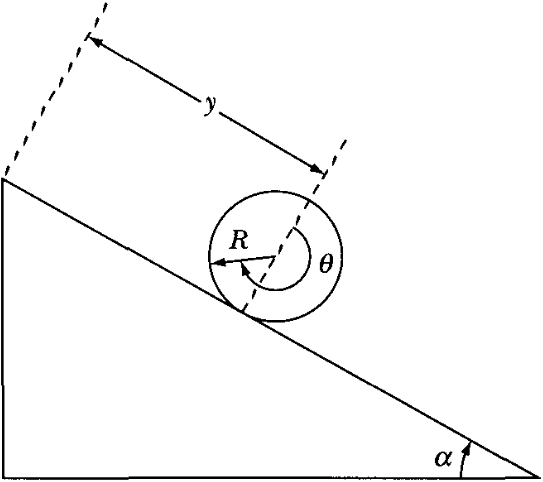
\includegraphics[width=\textwidth]{marion_fig6_7}
	\end{minipage}

	
	\item
	\begin{minipage}[t][7.5cm]{0.67\textwidth}
	\textbf{Doble máquina de Atwood} [Marion (e) ej. 7.8 y 7-37]\\
	Utilice el método de multiplicadores de Lagrange para encontrar las ecuaciones de movimiento y las tensiones de las cuerdas.
	\begin{enumerate}
		\item Verifique que obtiene las mismas aceleraciones generalizadas que se habían obtenido sin usar multiplicadores de Lagrange.
		Resultado:\\[5 pt]
		\(
			\ddot{y}_{1} = 
			\dfrac{2 g \left(2 m_{1} m_{2} + 2 m_{1} m_{3} + m_{1} m_{p} - 8 m_{2} m_{3} - 3 m_{2} m_{p} - 3 m_{3} m_{p} - m_{p}^{2}\right)}{4 m_{1} m_{2} + 4 m_{1} m_{3} + 2 m_{1} m_{p} + 16 m_{2} m_{3} + 8 m_{2} m_{p} + 8 m_{3} m_{p} + 3 m_{p}^{2}}\\[5 pt]
			\ddot{y}_{2} = 
			\dfrac{2 g \left(4 m_{1} + m_{p}\right) \left(m_{2} - m_{3}\right)}{4 m_{1} m_{2} + 4 m_{1} m_{3} + 2 m_{1} m_{p} + 16 m_{2} m_{3} + 8 m_{2} m_{p} + 8 m_{3} m_{p} + 3 m_{p}^{2}}
		\)
		\item Obtenga las tensiones de ambas cuerdas.
			Resultado:\\[5 pt]
			\(
				Q_{1} = \dfrac{g \left(- 32 m_{1} m_{2} m_{3} - 12 m_{1} m_{2} m_{p} - 12 m_{1} m_{3} m_{p} - 4 m_{1} m_{p}^{2} - 8 m_{2} m_{3} m_{p} - 3 m_{2} m_{p}^{2} - 3 m_{3} m_{p}^{2} - m_{p}^{3}\right)}{4 m_{1} m_{2} + 4 m_{1} m_{3} + 2 m_{1} m_{p} + 16 m_{2} m_{3} + 8 m_{2} m_{p} + 8 m_{3} m_{p} + 3 m_{p}^{2}}
				% Q_{1} = 
				% \dfrac{g \left(32 m_{1} m_{2} m_{3} + 12 m_{1} m_{2} m_{p} + 12 m_{1} m_{3} m_{p} + 4 m_{1} m_{p}^{2} + 8 m_{2} m_{3} m_{p} + 3 m_{2} m_{p}^{2} + 3 m_{3} m_{p}^{2} + m_{p}^{3}\right)}{4 m_{1} m_{2} + 4 m_{1} m_{3} + 2 m_{1} m_{p} + 16 m_{2} m_{3} + 8 m_{2} m_{p} + 8 m_{3} m_{p} + 3 m_{p}^{2}}
				\\[5 pt]
				Q_{2} = \dfrac{g m_{3} \left(- 16 m_{1} m_{2} - 4 m_{1} m_{p} - 4 m_{2} m_{p} - m_{p}^{2}\right)}{4 m_{1} m_{2} + 4 m_{1} m_{3} + 2 m_{1} m_{p} + 16 m_{2} m_{3} + 8 m_{2} m_{p} + 8 m_{3} m_{p} + 3 m_{p}^{2}}
				% Q_{2} = 
				% \dfrac{g m_{3} \left(16 m_{1} m_{2} + 4 m_{1} m_{p} + 4 m_{2} m_{p} + m_{p}^{2}\right)}{4 m_{1} m_{2} + 4 m_{1} m_{3} + 2 m_{1} m_{p} + 16 m_{2} m_{3} + 8 m_{2} m_{p} + 8 m_{3} m_{p} + 3 m_{p}^{2}}
			\)
		\end{enumerate}
	\end{minipage}
	\begin{minipage}[c][2cm][t]{0.3\textwidth}
		\begin{tikzpicture}
	
	% upper pulley
	\def \pulleyRadius {1.0};
	\coordinate (pulleyCentre) at (0,0);
	\fill [inner color = white, outer color = gray!25, thin] (pulleyCentre) circle (\pulleyRadius) node [below = 2 mm] {\(m_p\)};
	\filldraw (pulleyCentre) circle (1 mm);

	%% lower pulley dimensions
	\def \extra {0.4};
	\draw [-Latex] (pulleyCentre) ++(110:{\pulleyRadius + \extra / 2}) arc (110 : 160 : {\pulleyRadius + \extra / 2 }) node [midway, above] {\(\theta_1\)};
	
	
	% dashed lines from 0.1 at each side of the circle
	\def \deltax {1.0};
	\draw [dashed] (0.2,0) -- ({\pulleyRadius + 2* \deltax},0);
	\draw [dashed] (-0.2,0) -- ({-\pulleyRadius - \deltax},0);
	\node at ({\pulleyRadius / 2}, 0) [above] {\(R\)};

	% weight m_1
	\def \boxwidth {\pulleyRadius/ 2.5};
	\def \boxAheight {-1.5};
	\shade [ball color=black!80] (-\pulleyRadius, \boxAheight) circle (\boxwidth) node {\color{white} $m_1$};
	
	% lower pulley
	\def \lowerPulleyHeight {-2.5};
	\coordinate (lowerPulleyCentre) at (\pulleyRadius,\lowerPulleyHeight);
	\fill [inner color = white, outer color = gray!25, thin] (lowerPulleyCentre) circle (\pulleyRadius) node [below = 2mm] {\(m_p\)};
	% \shade [ball color=black!80] (\pulleyRadius, \lowerPulleyHeight) circle (\boxwidth) node {\color{white} $m_2$};
	\filldraw (lowerPulleyCentre) circle (1 mm);
	\node at ($(lowerPulleyCentre) + ({\pulleyRadius / 2}, 0) $) [above] {\(R\)};
	
	%% lower pulley dimensions
	\draw [-Latex] (lowerPulleyCentre) ++(110:{\pulleyRadius + \extra / 2}) arc (110 : 160 : {\pulleyRadius + \extra / 2 }) node [midway, above] {\(\theta_2\)};
	
	% rope 1
	\draw [ultra thick] (-\pulleyRadius, \boxAheight + \boxwidth) -- (-\pulleyRadius,0);
	\draw [ultra thick] ( \pulleyRadius, \lowerPulleyHeight) -- (\pulleyRadius,0); 
	\draw [ultra thick] (pulleyCentre) ++(0:\pulleyRadius) arc (0:180:\pulleyRadius) node [above left] {\(\ell_1\)};


	% rope 2
	\draw [ultra thick] (lowerPulleyCentre) ++(0:\pulleyRadius) arc (0:180:\pulleyRadius) node [above left] {\(\ell_2\)};
	\def \belowPulley3 {-1.5};
	\coordinate (weight3) at ($(lowerPulleyCentre) + ( \pulleyRadius , \belowPulley3 )$);  
	\draw [ultra thick] ($(lowerPulleyCentre) + (\pulleyRadius , 0) $) -- (weight3);
	
	\def \belowPulleyHeight2 {-2.0};
	\coordinate (weight2) at ($(lowerPulleyCentre) + ( -\pulleyRadius , \belowPulleyHeight2 )$);  
	\draw [ultra thick] ($(lowerPulleyCentre) + (-\pulleyRadius , 0) $) -- (weight2);

	% weight m_3
	\shade [ball color=black!80] (weight3) circle (\boxwidth) node {\color{white} $m_3$};

	% weight m_2
	\shade [ball color=black!80] (weight2) circle (\boxwidth) node {\color{white} $m_2$};


	% upper puley dimensions
	\def \pendeLeft {-\pulleyRadius - \boxwidth - 0.2};
	\def \pende {\pulleyRadius + \boxwidth + 0.2};
	\def \pendePulley {2* \pulleyRadius + 0.2};
	\draw [-Latex] (\pendeLeft, 0) -- (\pendeLeft, \boxAheight) node [midway, left] {\(y_1\)};
	\draw [-Latex] ( \pendePulley, 0) -- ( \pendePulley, \lowerPulleyHeight) node [midway, right] {\(y_p\)};


	% lower pulley dimensions
	\draw [-Latex] ($(lowerPulleyCentre) + (\pendeLeft, 0) $) -- ($(lowerPulleyCentre) + (\pendeLeft, \belowPulleyHeight2 ) $) node [midway, left] {\(y_2\)};
	\draw [-Latex] ($(lowerPulleyCentre) + (\pende, 0) $) -- ($(lowerPulleyCentre) + (\pende, \belowPulley3 ) $) node [midway, right] {\(y_3\)};

	
	% lower pulley dashed lines
	\draw [dashed] ($ (lowerPulleyCentre) + (-0.2,0) $) -- ($ (lowerPulleyCentre) + ({-\pulleyRadius - \deltax},0) $);
	\draw [dashed] ($ (lowerPulleyCentre) + (0.2,0)$) -- ($(lowerPulleyCentre) + ({\pulleyRadius + \deltax},0) $);

	% ceiling
	\def \ceilingAbove {1.5};
	\draw [line width = 1 mm] ($(pulleyCentre) + (0,\ceilingAbove)$) -- (pulleyCentre);
	\draw [ultra thick] ($(pulleyCentre) + ({- \pulleyRadius},\ceilingAbove)$)  -- ($(pulleyCentre) + (\pulleyRadius,\ceilingAbove)$);
	\fill [pattern = north east lines] ($(pulleyCentre) + ({- \pulleyRadius},\ceilingAbove)$)  rectangle ($(pulleyCentre) + (\pulleyRadius, {\ceilingAbove + 0.2 })$);


\end{tikzpicture}
		% 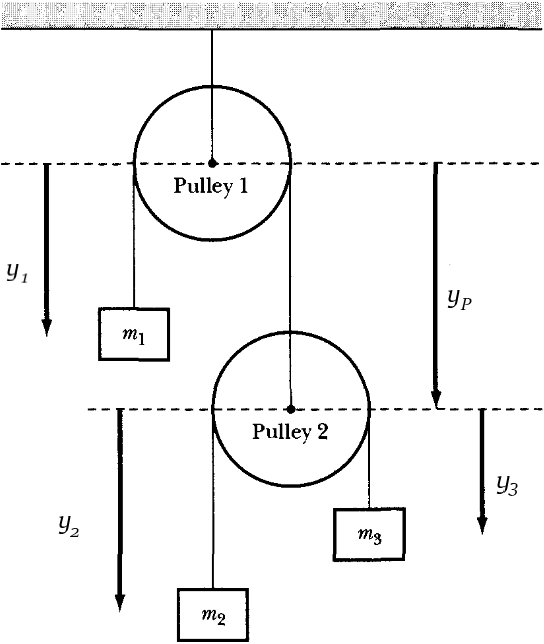
\includegraphics[width=\textwidth]{marion_fig7_6}
	\end{minipage}

	% \newpage

	\item
	\begin{minipage}[t][7.5cm]{0.65\textwidth}
		\textbf{Pesos enlazados por una cuerda} [Taylor 7.50]\\
		Una partícula de masa \(m\), situada sobre una mesa horizontal sin fricción, está unida mediante una cuerda ideal de longitud \(\ell\) a otra partícula de masa \(M\).
		La cuerda pasa por un orificio practicado en la mesa, el cual no presenta rozamiento.
		La segunda pesa pende vertical con una distancia por debajo de la mesa \(d = \ell - \rho\), función de la distancia de la primera al hueco, \(\rho\).
		\begin{enumerate}
			\item Asumiendo que \(\theta\) no es necesariamente constante obtenga las ecuaciones de Lagrange para \(\rho\) y \(d\). Resultado:\\[5 pt]
			\(M \left(- g + \ddot{d}\right) = \lambda_{1} \qquad m \left(- \rho \dot{\varphi}^{2} + \ddot{\rho}\right) = \lambda_{1}\)
			\item Resuelva el sistema para \(\rho, y\) y el multiplicador de Lagrange \(\lambda_1\) encontrando las fuerzas de tensión sobre ambas masas.\\[5 pt]
			Resultado: \(Q_{\rho} = - \dfrac{M m \left(g + \rho \dot{\varphi}^{2}\right)}{M + m}\)
		\end{enumerate}
	\end{minipage}
	\begin{minipage}[c][-1cm][t]{0.3\textwidth}
		\begin{tikzpicture}
    % Perspective transformation
    \def\angleX{45} % Angle for the X-axis
    \def\extentBack{3}  % Angle for the Y-axis
    
    % Coordinates of the table's corners
    \coordinate (A) at (0, 0);
    \coordinate (B) at ($(A)+(4,0)$); 
    \coordinate (C) at ($(B)+(\angleX:\extentBack)$);
    \coordinate (D) at ($(A)+(\angleX:\extentBack)$);

    % Draw the table in perspective
    \filldraw[gray!30] (A) -- (B) -- (C) -- (D) -- cycle; % Top surface
    \draw (A) -- (B); % Front edge
    \draw (B) -- (C); % Side edge
    \draw (C) -- (D); % Back edge
    \draw (A) -- (D); % Left edge

    % Centre point of rotation on the table (O)
    \coordinate (O) at ($(A)!0.5!(C)$); % Midpoint between A and B
 
 		% while ellipse at top surface middle
		\filldraw[white] (O) ellipse (0.2 and 0.1);

		% rotate a draw line by \rotationAngle
		\def \rotationAngle {30}
		\def \radius {1.3}
	
		% dashed lines
		\draw[dashed] (O) --  ($(O) + (2 * \radius,0)$);
		\draw[dashed, rotate around={\rotationAngle:(O)}] (O) --  ($(O) + (2 * \radius,0)$);

	  % Draw theta angle arc
		\draw[thick, -Latex] ($(O) + (1.75* \radius,0)$) arc[start angle=0, end angle= \rotationAngle, radius= 1.75* \radius] node[midway, right] {$\theta$};

		% rope	
		\draw[ultra thick, rotate around={\rotationAngle:(O)}] (O) -- ($(O)+ (\radius, 0)$) node[midway, above left] {$\rho$};

		% over table weight
		\shade[ball color =black!80, rotate around={\rotationAngle:(O)}] ($(O)+ (\radius, 0)$) circle (0.25) node[] {\color {white} $m$};
	
    % Draw the hanging mass and the string (l- r)
    \coordinate (massPoint) at ($(O)-(0,2.8)$);
    \draw[ultra thick] (O) -- (massPoint) node[midway, right] {$\ell$};
    % \filldraw[black] (massPoint) circle (3pt) node[right] {$M$};
		\shade [ball color=black!80] (massPoint) circle(0.25) node [] {\color{white} $M$};

\end{tikzpicture}
		% 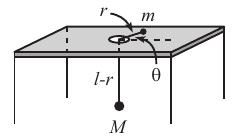
\includegraphics[width=\textwidth]{cmchap6_fig6_5}
	\end{minipage}


	\item
	\begin{minipage}[t][4.5cm]{0.62\textwidth}
		\textbf{Partícula deslizando sobre una semiesfera} [Marion (e) ex. 7.10]\\
		La partícula de masa \(m\), considerada puntual, desliza sobre una semiesfera de radio \(R\) sin fricción.
		\begin{enumerate}
			\item Encuentre la fuerza de la ligadura.\\
			Resultado: \(Q_{\rho} = m \left(- R \dot{\theta}^{2} + g \cos{\left(\theta \right)}\right)\)
			\item Calcule el ángulo en que la partícula se despega de la semiesfera.\\
			Resultado: \(\theta^\mathrm{despegue} \approx 48.19^\circ\) 
		\end{enumerate}
	\end{minipage}
	\begin{minipage}[c][0cm][t]{0.3\textwidth}
		\begin{tikzpicture}[scale= 1.0]
  \draw [ultra thick] (-3,0) -- (3,0);
  % \draw [ultra thick] (-3,0) -- (3,0);
  \fill [pattern = north east lines] (-3,0) rectangle (3,-0.2); % piso
  \draw [ultra thick] (-2,0) .. controls (-2,2*0.555) and (-2*0.555,2) .. (0,2) .. controls (2*0.555,2) and (2,2*0.555) .. (2,0); % semi esfera
  % \filldraw (0,2.2) circle (0.2); % masa superior
  % \fill (2*0.5+.12,1.732+.18) circle [radius=0.25] node [midway, text=white] { \( m \) };
  % \filldraw (2*0.5+.12,1.732+.18) circle (0.2) node [above, right=5] {\(m\)}; % masa a la derecha
  \shade [ball color=black!80] (2*0.5+.12,1.732+.18) circle(0.2) node [] {\color{white} $m$};
  % \draw (2,2) circle [radius=0.3, color=white, fill=black] node {$T_1$};
  \draw [dashed] (0,0) -- (0,2.5); % linea vertical
  \draw [-Latex] (0,0) -- (1,1.732) node [midway, anchor=west] {\(R\)}; % linea hacia la derecha
  \draw [-Latex] (0,1) arc (90:60:1) node [above left] {\(\theta\)}; % arco c/ flecha comenzando en (0,1), de 90 a 60 grados, 1...
  % \node [circle,draw,label=60:$60^\circ$,label=below:$-90^\circ$] {\(m\)}; 
  % \node at (-2*0.5+.15,1.732+.15) [circle,draw,fill=black] {\(m\)}; 
  \draw [-Latex, thick] (-2.5,2) -> (-2.5,1) node [above=15, right=2] {\(\vec{g}\)}; % g vertical
\end{tikzpicture}
		% \includegraphics[width=\textwidth]{marion7_10}
	\end{minipage}
	
	Para llegar al ángulo de despegue debe resolver la ecuación diferencial a la que arribará tras resolver la problemática de las fuerzas de ligadura, que será $\ddot{\theta} = \dfrac{g \sin(\theta)}{R}$.
	Esta expresión es integrable para el recorrido que hace la partícula.
	Para facilitar esto se intercala por regla de la cadena derivaciones en función de \(\theta\) en la definición de la aceleración.
	$$
		\ddot{\theta} 
		= \frac{d \dot{\theta} }{d t} 
		= \frac{d \theta}{d t} \frac{d \dot{\theta}}{d \theta} 
		= \dot{\theta} \frac{d \dot{\theta}}{d \theta}
	$$

	Como la partícula parte de $\theta(t=0) = 0$ con $\dot{\theta}(t=0) = 0$.
	$$
	\begin{aligned}
		\ddot{\theta} = \dot{\theta} \frac{d \dot{\theta}}{d \theta}
		&= \frac{g}{R} \sin(\theta)\\
		\dot{\theta} d \dot{\theta}
		&= \frac{g}{R} \sin(\theta) d \theta \\
		\int_0^{\dot{\theta}_\mathrm{despegue}} \dot{\theta} d \dot{\theta}
		&= \frac{g}{R} \int_0^{\theta_\mathrm{despegue}} \sin{\theta} d \theta\\
		\frac{\dot{\theta}^2}{2} \bigg|_0^{\dot{\theta}_\mathrm{despegue}}
		&= \frac{g}{R} (-\cos{\theta}) \bigg|_0^{\theta_\mathrm{despegue}}\\
		\frac{\dot{\theta}_\mathrm{despegue}^2}{2}
		&= \frac{g}{R} (-\cos(\theta_\mathrm{despegue}) + 1)\\
	\end{aligned}
	$$
	Con esto hay que substituir $\dot{\theta}^2$ en una expresión de $F^\mathrm{ligadura}_{\rho}$, que debe ser nula en el momento de despegue.


\end{enumerate}

\end{document}
